\documentclass[a4paper,11pt]{exam}
\printanswers % pour imprimer les réponses (corrigé)
%\noprintanswers % Pour ne pas imprimer les réponses (énoncé)
\addpoints % Pour compter les points
% \noaddpoints % pour ne pas compter les points
%\qformat{\textbf{\thequestion ) } }
%\qformat{\textbf{\thequestion )} (\thepoints) \\} % Pour définir le style des questions (facultatif)
\usepackage{color} % définit une nouvelle couleur
\shadedsolutions % définit le style des réponses
% \framedsolutions % définit le style des réponses
\definecolor{SolutionColor}{rgb}{0.8,0.9,1} % bleu ciel
\renewcommand{\solutiontitle}{\noindent\textbf{Solution:}\par\noindent} % Définit le titre des solutions




\makeatletter

\def\maketitle{{\centering%
	\par{\huge\textbf{\@title}}%
	\par{\@date}%
	\par}}

\makeatother

\lhead{NOM Pr\'enom :}
\rhead{\textbf{Les r\'eponses doivent \^etre justifi\'ees}}
\cfoot{\thepage / \pageref{LastPage}}


%\usepackage{../../pas-math}
%\usepackage{../../moncours}


%\usepackage{pas-cours}
%-------------------------------------------------------------------------------
%          -Packages nécessaires pour écrire en Français et en UTF8-
%-------------------------------------------------------------------------------
\usepackage[utf8]{inputenc}
\usepackage[frenchb]{babel}
\usepackage[T1]{fontenc}
\usepackage{lmodern}
\usepackage{textcomp}



%-------------------------------------------------------------------------------

%-------------------------------------------------------------------------------
%                          -Outils de mise en forme-
%-------------------------------------------------------------------------------
\usepackage{hyperref}
\hypersetup{pdfstartview=XYZ}
%\usepackage{enumerate}
\usepackage{graphicx}
\usepackage{multicol}
\usepackage{tabularx}
\usepackage{multirow}


\usepackage{anysize} %%pour pouvoir mettre les marges qu'on veut
%\marginsize{2.5cm}{2.5cm}{2.5cm}{2.5cm}

\usepackage{indentfirst} %%pour que les premier paragraphes soient aussi indentés
\usepackage{verbatim}
\usepackage{enumitem}
\usepackage[usenames,dvipsnames,svgnames,table]{xcolor}

\usepackage{variations}

%-------------------------------------------------------------------------------


%-------------------------------------------------------------------------------
%                  -Nécessaires pour écrire des mathématiques-
%-------------------------------------------------------------------------------
\usepackage{amsfonts}
\usepackage{amssymb}
\usepackage{amsmath}
\usepackage{amsthm}
\usepackage{tikz}
\usepackage{xlop}
%-------------------------------------------------------------------------------



%-------------------------------------------------------------------------------


%-------------------------------------------------------------------------------
%                    - Mise en forme avancée
%-------------------------------------------------------------------------------

\usepackage{ifthen}
\usepackage{ifmtarg}


\newcommand{\ifTrue}[2]{\ifthenelse{\equal{#1}{true}}{#2}{$\qquad \qquad$}}

%-------------------------------------------------------------------------------

%-------------------------------------------------------------------------------
%                     -Mise en forme d'exercices-
%-------------------------------------------------------------------------------
%\newtheoremstyle{exostyle}
%{\topsep}% espace avant
%{\topsep}% espace apres
%{}% Police utilisee par le style de thm
%{}% Indentation (vide = aucune, \parindent = indentation paragraphe)
%{\bfseries}% Police du titre de thm
%{.}% Signe de ponctuation apres le titre du thm
%{ }% Espace apres le titre du thm (\newline = linebreak)
%{\thmname{#1}\thmnumber{ #2}\thmnote{. \normalfont{\textit{#3}}}}% composants du titre du thm : \thmname = nom du thm, \thmnumber = numéro du thm, \thmnote = sous-titre du thm

%\theoremstyle{exostyle}
%\newtheorem{exercice}{Exercice}
%
%\newenvironment{questions}{
%\begin{enumerate}[\hspace{12pt}\bfseries\itshape a.]}{\end{enumerate}
%} %mettre un 1 à la place du a si on veut des numéros au lieu de lettres pour les questions 
%-------------------------------------------------------------------------------

%-------------------------------------------------------------------------------
%                    - Mise en forme de tableaux -
%-------------------------------------------------------------------------------

\renewcommand{\arraystretch}{1.7}

\setlength{\tabcolsep}{1.2cm}

%-------------------------------------------------------------------------------



%-------------------------------------------------------------------------------
%                    - Racourcis d'écriture -
%-------------------------------------------------------------------------------

% Angles orientés (couples de vecteurs)
\newcommand{\aopp}[2]{(\vec{#1}, \vec{#2})} %Les deuc vecteurs sont positifs
\newcommand{\aopn}[2]{(\vec{#1}, -\vec{#2})} %Le second vecteur est négatif
\newcommand{\aonp}[2]{(-\vec{#1}, \vec{#2})} %Le premier vecteur est négatif
\newcommand{\aonn}[2]{(-\vec{#1}, -\vec{#2})} %Les deux vecteurs sont négatifs

%Ensembles mathématiques
\newcommand{\naturels}{\mathbb{N}} %Nombres naturels
\newcommand{\relatifs}{\mathbb{Z}} %Nombres relatifs
\newcommand{\rationnels}{\mathbb{Q}} %Nombres rationnels
\newcommand{\reels}{\mathbb{R}} %Nombres réels
\newcommand{\complexes}{\mathbb{C}} %Nombres complexes


%Intégration des parenthèses aux cosinus
\newcommand{\cosP}[1]{\cos\left(#1\right)}
\newcommand{\sinP}[1]{\sin\left(#1\right)}


%Probas stats
\newcommand{\stat}{statistique}
\newcommand{\stats}{statistiques}
%-------------------------------------------------------------------------------

%-------------------------------------------------------------------------------
%                    - Mise en page -
%-------------------------------------------------------------------------------

\newcommand{\twoCol}[1]{\begin{multicols}{2}#1\end{multicols}}


\setenumerate[1]{font=\bfseries,label=\textit{\alph*})}
\setenumerate[2]{font=\bfseries,label=\arabic*)}


%-------------------------------------------------------------------------------
%                    - Elements cours -
%-------------------------------------------------------------------------------





%\usepackage{fullpage}
\author{\ }
\date{?}
\title{$6^e C$ : DS num\'ero 5}


\begin{document}
%	\usepackage{fancyhdr}
%	
%	\pagestyle{fancy}
%	\fancyhf{}
	%\rhead{Share\LaTeX}

	\maketitle
	
\begin{center}
	\textbf{Calculatrice interdite, le soin et la qualité de la rédaction seront pris en compte}
\end{center}

\begin{small}
	\begin{center}
		\begin{tabular}{|@{\ }l@{\ }|@{\ }c@{\ }|@{\ }c@{\ }|@{\ }c@{\ }|@{\ }c@{\ }|}
			\hline
			\textbf{Compétence} & \textbf{MI} & \textbf{MF} & \textbf{MS} & \textbf{TBM} \\
			\hline
			\textbf{Calculer} (Calculer avec des nombres décimaux. ) &  \ \ & \ \ & \ \ & \ \  \\
			\hline	
			\textbf{Calculer} (Contrôler la vraisemblance de ses résultats.) & \ \ & \ \ &  \ \  & \ \ \\
			\hline
			\textbf{Modéliser} ( Résolution de problèmes de la vie courante. ) &  \ \ & \ \ & \ \ & \ \  \\
			\hline
		\end{tabular}
	\end{center}
\end{small}	

	
	
	

%\newpage

\section{Multiples et diviseurs}

\begin{questions}
	\question Qu'est ce qu'un nombre pair ?
	
	\question Parmi les nombres ci-dessous, donner en justifiant la réponse : 	
	\begin{itemize}
		\begin{multicols}{2}
			\item 153
			\item 42
			\item 3525
			\item \num{21729}
			\item 180
		\end{multicols}
	\end{itemize}


	\begin{parts}
		\begin{multicols}{3}
			\part les multiples de 3.
		\part les multiples de 5.
		\part les multiples de 9.
		\end{multicols}
	\end{parts}

	\question Donner, en justifiant la réponse, deux nombres qui sont divisibles à la fois par 2, 10 et 3.
\end{questions}

%\section{Spectacle (3 points)}

Pour le spectacle de fin d'année, la maîtresse a placé 7 élèves de ma classe de CE2 comme sur le schéma ci-dessous.

\begin{center}
	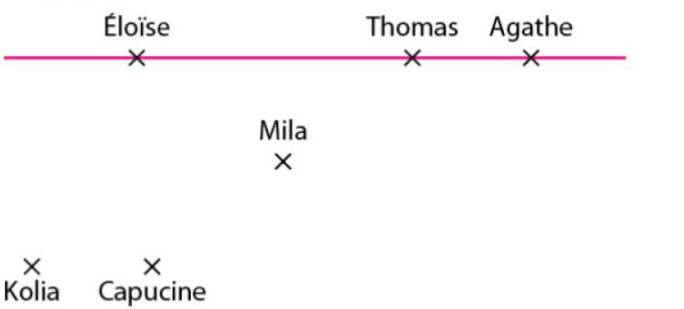
\includegraphics[scale=0.5]{img/spectacle}
\end{center}

Elle veut que la position des élèves soit symétrique par rapport à celle de Mila.

\begin{questions}
	\question[1\half] En utilisant uniquement une règle non graduée, déterminer la position d'Eneko, le dernier élève à ne pas avoir encore été placé. Laisser apparents les traits de construction.
	
	\begin{solution}
		\begin{center}
			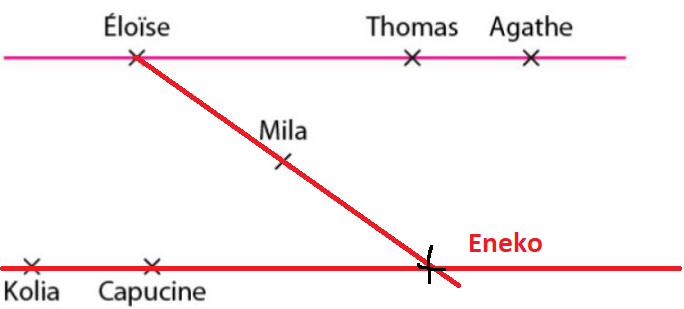
\includegraphics[scale=0.5]{img/spectacle_corr}
		\end{center}
	\end{solution}
	
	\question[1\half] Quelle propriété permet de répondre à la question ?
	\begin{solution}
		On sait que \'Eloïse, Thomas et Agathe sont alignés,
		or le symétrique d'une droite par rapport à un point est une autre droite. 
		Donc Kolia, Capucine et Thomas seront aussi alignés.
	\end{solution}
\end{questions}

%\subsection{Definition}

\begin{mydef}
	
	\iftoggle{eleve}{%
		Effectuer la \hrulefill 
		
		\vspace*{0.2cm}
		\hrulefill 
		
		\vspace*{0.2cm}
		\hrulefill 
		
		
		\vspace*{0.2cm}
		\hrulefill 
		
		
		\vspace*{0.2cm}
		\hrulefill 
		
		
		\vspace*{0.2cm}
		\hrulefill 
	}{%
		Effectuer la \kw{division euclidienne} d’un nombre entier, appelé \kw{dividende}, par un nombre entier, différent de zéro, appelé \kw{diviseur}, c’est trouver deux autres nombres entiers, le \kw{quotient} et le \kw{reste}, tels que : 
		
		\begin{equation*}
			diviseur \times quotient + reste = dividende	
		\end{equation*}
	}
	

	
\end{mydef}


\iftoggle{eleve}{%
	\begin{center}
		$\begin{array}{c|c}
			 &  \hspace*{2cm} \\
			\cline{2-2}
			&  \\
			 & \\
		\end{array}$
	\end{center}
}{%
	\begin{center}
		$\begin{array}{c|c}
			Dividende & Diviseur \\
			\cline{2-2}
			& Quotient \\
			Reste & \\
		\end{array}$
	\end{center}
}


%\begin{mywarning}
%	On ne peut pas diviser par 0.
%\end{mywarning}

%\subsection{Technique de division}

%\begin{mymeth}
%\vspace*{-1cm}	

%\begin{mymethname}{Technique de division}
%\begin{multicols}{2}
%	\begin{center}
%%		$\begin{array}{rc|c}
%%		731 & & 34 \\
%%		\cline{3-3}
%%		51& & 21 \\
%%		17 & & \\
%%		\end{array}$
%		\opidiv{731}{34}
%	\end{center}
%
%Conclusion : $34 \times 21 + 17 = 731$
%\end{multicols}
%
%
%Le diviseur 34 a deux chiffres, on commence la division avec les deux premiers chiffres du dividende $73 > 34 $; 
%combien de fois 34 dans 73 : 2 fois ; on soustrait $2 \times 34$ à 73.
%
%On abaisse le 1. 
%Combien de fois 34 dans 51 : 1 fois ; 
%on soustrait $1 \times 34$ à 51 ; $17 < 34$ ; on a fini.\\
%
%
%\textbf{\underline{Vérification:}}\\
%Il existe un moyen pour vérifier si une division euclidienne est juste. 
%Pour cela, on multiplie le quotient par le diviseur, puis on ajoute le reste. 
%Si le résultat obtenu est égal au dividende, la division est juste.
%\end{mymethname}


\begin{myexs}
	Poser et vérifier les divisions euclidiennes suivantes :  $653 \div 7$ et $73 \div 5$
	
	\vspace*{4cm} 
\end{myexs}

%\begin{mypb}
%	Dans une classe de 26 élèves, on forme des équipes de volley-ball (6 joueurs par équipe).
%	
%	\begin{enumerate}
%		\item Combien d’équipes forme-t-on ?
%		\item Combien y-a-t-il de remplaçants ?	
%	\end{enumerate}
%
%\vspace*{5cm} 	
%\end{mypb}

\section{Division décimale}


\begin{questions}
	\question Poser et calculer la valeur exacte des quotients suivants :
	
	\begin{parts}
		\begin{multicols}{3}
			\part $\num{4.50} \div 9$
			\part $\num{4.20} \div 4$
			\part $\num{31.40} \div 10$
		\end{multicols}
	\end{parts} 
	
	\question Répondre par une phrase aux questions ci-dessous :
	
	\begin{parts}
		\part Quatre ampoules sont vendues \num{4.20} €. Quel est le prix d'une ampoule ?
		
		\part Dix mètres de câble sont vendus \num{31.40} €. Quel est le prix d'un mètre de câble ?
		
		\part Neuf feutres identiques coûtent \num{4.50} €. Quel est le prix de chaque feutre ?
	\end{parts}
	 
	
	
\end{questions}

\section{Problème}

Justine est dans la file de skieurs qui attendent pour monter dans un téléphérique. 135 personnes sont devant elle. Il est 9h20 et un téléphérique arrive. Chaque téléphérique embarque 24 passagers. On attend 10 minutes entre les départs de deux téléphériques.

\begin{questions}
	\question Combien de téléphériques vont partir sans Justine ?
	
	\question \'A quelle heure Justine montera-t-elle dans le téléphérique ?
\end{questions}
\label{LastPage}

%\section{Consommation électrique}
%
%Une consommation d'électricité se mesure en 
\end{document}